\newpage
\section{Auswertung}
\label{sec:auswertung}
\subsection{B-Feld Messung}
Da der Zeemann Effekt abhängig vom angelegten B-Feld ist un in diesem Versuchsaufbau nur der Spulenstrom zur Magnetfelderzeugung eingestellt werden kann muss zunächst der Zusammenhang zwischen Spulenstrom und Magnetfeld betrachtet werden.
Mit den Werten die wie in Abschnitt \ref{sec:BFeld} aufgenommen wurden wird ein linearer Fit und ein Fit eines Polynoms dritter Ordnung durchgeführt.\\
\begin{figure}[ht]
    \center
    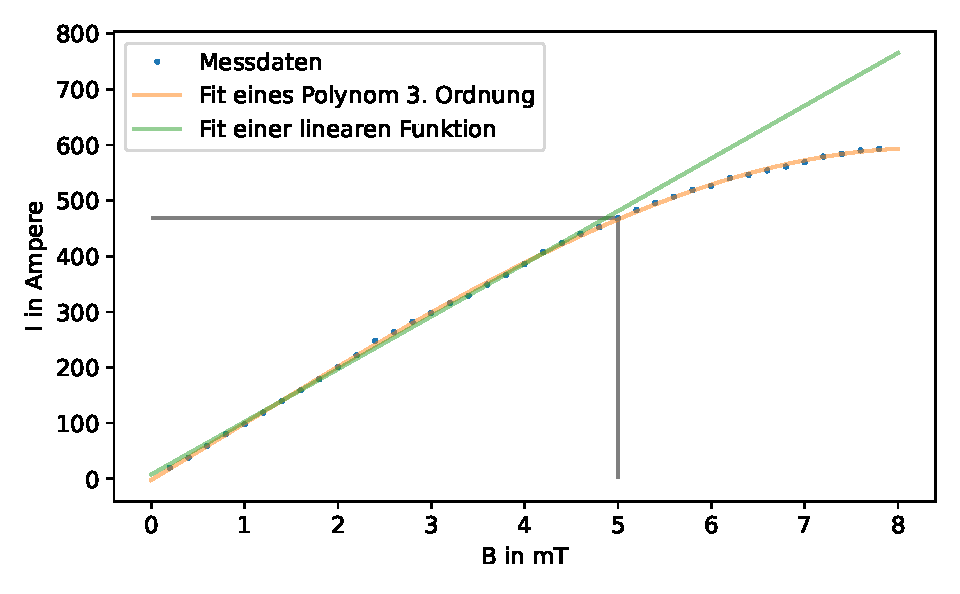
\includegraphics[width=0.65\textwidth]{plots/B_Feld.pdf}
    \caption{Die Feldstärke wird gegen den angelegten Spulenstrom aufgetragen. Im Bereich des grauen Kastens }
    \label{fig:B_Feld}
\end{figure}
Die beiden Fits basieren dabei auf folgenden Funktionen:
\begin{align*}
    B_1(I) &= aI^3+bI^2+cI+d\\
    B_2(I) &= mI+e
\end{align*}
Dabei ergeben sich die Parameter zu:
\begin{align*}
    a &= \SI[per-mode = fraction]{-0.62 +- 0.05}{\tesla \per \cubic \ampere}\\
    b &= \SI[per-mode = fraction]{1.7+-0.6}{\tesla \per \square \ampere}\\
    c &= \SI[per-mode = fraction]{100.8+-2.2}{\tesla \per \ampere}\\
    d &= \SI[per-mode = fraction]{-2.1+-2.1}{\tesla}\\
    \\
    m &= \SI[per-mode = fraction]{94.7+-0.9}{\tesla \per \ampere}\\
    e &= \SI[per-mode = fraction]{7.6+-2.6}{\tesla}\\ 
\end{align*}
\subsection{Blau senkrecht}
\subsection{Rot senkrecht}